\begin{blocksection}

\textbf{\underline{Control Logic}}

A controller send signals to our circuit, telling which pieces to perform what operations.  Not all control signals matter for every instruction: for example, R-type instructions ignores the output from the immediate generator.  Control signals are used to pick between mux inputs in order to perform the correct operation.  They are embedded within the actual machine code for an instruction.

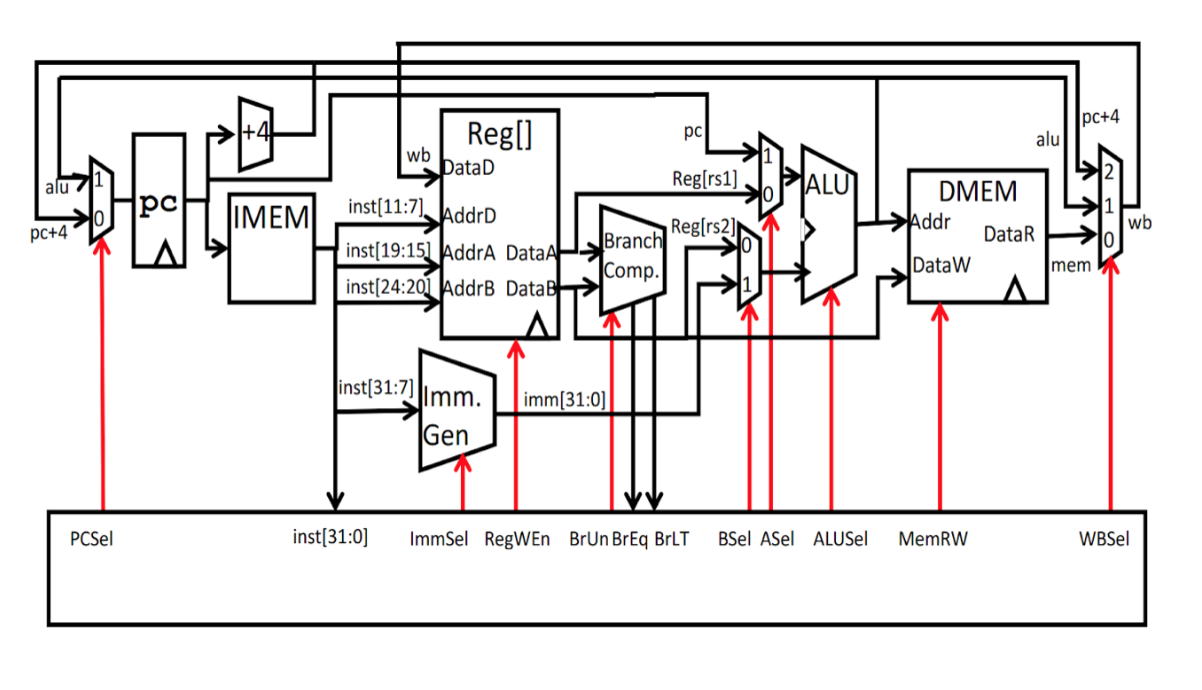
\includegraphics[width=\textwidth]{singlecycle/explanation_2}

\textbf{Control Inputs}
\newline
\newline
\begin{tabular}{ |l|l|l|l| } 
 \hline
 \textbf{Signal:} & \textbf{inst[31:0]} & \textbf{BrEq} & \textbf{BrLT} \\ 
 \hline
 Purpose: & Sends the current instruction to control & (DataA == DataB) ? 1 : 0 & (DataA < DataB) ? 1 : 0 \\ 
 \hline
\end{tabular}

\bigskip
\textbf{Control Outputs}
\newline
\newline
\begin{tabular}{ |l|l|l|l|l| } 
 \hline
 \textbf{Signal:} & \textbf{PCSel} & \textbf{ALUSel} & \textbf{RegWEn} & \textbf{ImmSel} \\ 
 \hline
 Purpose: & Next instruction location. & What operation to perform. & Do we change a register’s value? & Format the immediate properly. \\ 
 \hline
 \textbf{Signal:} & \textbf{MemRW} & \textbf{WBSel} & \textbf{BrUn} & \textbf{ASel/BSel} \\
 \hline 
 Purpose: & Read or write to mem. & What value to write back. & Branch signed or unsigned & Pick between the inputs for ALU \\
 \hline
\end{tabular}

\end{blocksection}